\problem

En una loter{\'\i}a de 100 billetes hay 2 que tienen premio.
\begin{enumerate}
	\item ?`Cu{\'a}l es la probabilidad de ganar al menos un premio si  se  compran
	12 billetes?
	\item ?`Cuantos billetes habr{\'a} que comprar  para  que  la  probabilidad  de
	ganar al menos un  premio sea mayor que 4/5?
\end{enumerate}

\subproblem
Sea A el suceso de ganar al menos un premio si se compran 12 billetes. Para determinarlo, procedemos primero a calcular $P(\bar A)$ mediante la regla de Laplace en cada boleto de lotería comprado:
	
	$$
		P(\bar A) = \frac{98}{100}·\frac{97}{99}·\frac{96}{98}...\frac{98-12+1}{100-12+1} = 0,77333
	$$
	
	Por tanto, deducimos que: 
	$$
	 P(A) = 0,22667 
	$$
	
	\subproblem
	
	Para calcular el número de boletos de lotería que se ha de adquirir para que se alcance dicha probabilidad, sea $A_n$ el suceso de ganar al menos un premio tras adquirir n billetes de lotería. Queremos hallar $n \in \mathbb{N}$ de forma que se verifique $P(A_n) = \frac{4}{5} > 0,8$, por lo que 
	se ha de cumplir $P(\bar A_n) < 0,2$. Razonamos nuevamente como el apartado anterior:
	
	$$
	P(\bar A_n) = \frac{98}{100}·\frac{97}{99}·\frac{96}{98}...\frac{98-n+1}{100-n+1} = \frac{(99-n+1)·(98-n+1)}{100·99} < 0,2
	$$

	\begin{figure}[h]
		\centering
		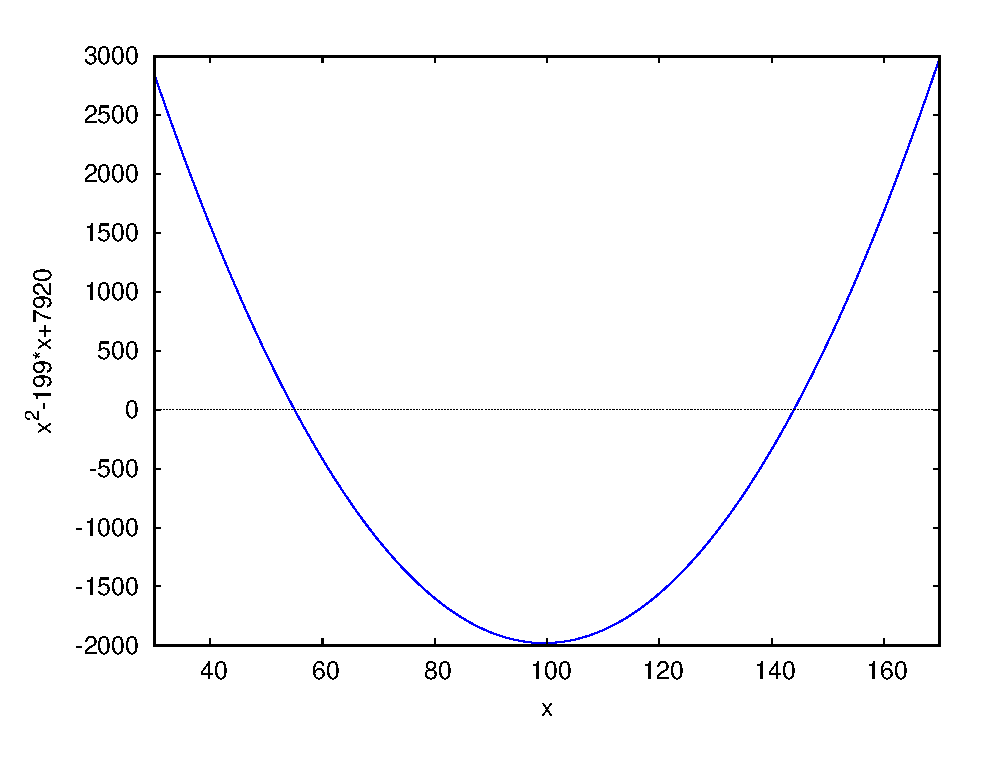
\includegraphics[scale=0.40]{ejercicio-6-grafica.eps}
	\end{figure}
	
		
	
	De la desigualdad de la derecha obtenemos que se ha de cumplir $n^2 -199·n + 7920 < 0$. Dado que la función $f(x) = x^2 -199·x + 7920$ corta al eje OX en los puntos $x=55$ y $x=144$ y es cóncava hacia arriba, deducimos que la mínima cantidad de boletos que ha de adquirir una persona para tener una probabilidad estrictamente mayor que 0,8 son \textbf{56 boletos}.